\setAuthor{Konstantin Dukatš}
\setRound{piirkonnavoor}
\setYear{2024}
\setNumber{G 9}
\setDifficulty{9}
\setTopic{TODO}

\prob{Laetud kuul}
\begin{wrapfigure}{r}{0.3\textwidth}
  \vspace{-25pt}
  \begin{center}
  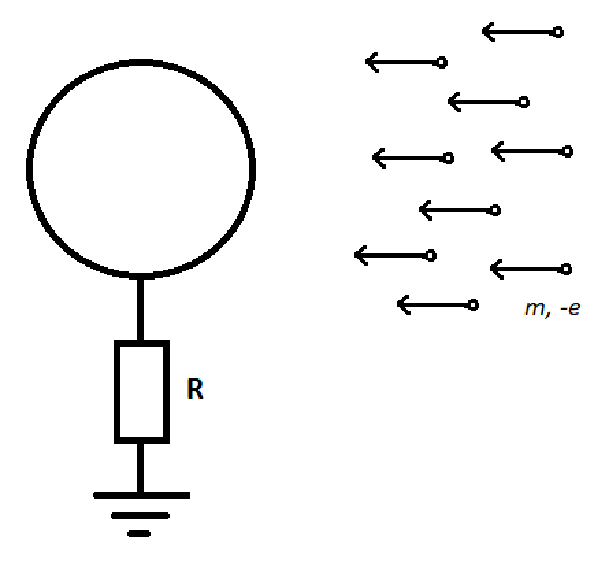
\includegraphics[width=\linewidth]{2024-v2g-09-yl.png}
  \vspace{-30pt}
  \end{center}
\end{wrapfigure}



Metallist kuul raadiusega $a$ on maandatud takistuse $R$ kaudu, vt joonist. Kuulile on suunatud lai elektronide (mass $m$, laeng $-e$) voog, kus elektronide kiirus on $v$ ja elektronide arv ruumalaühiku kohta on  $n$. Millise laengu omandab kuul tasakaalulise olukorra saabudes? Elektronide kiirus on nii suur, $v \gg n e^2 a^2 R / m$, et kuulile kogunev laeng ei suuda nende trajektoori märkimisväärselt kõverdada. Arvtihedus $n$ on nii väike, et elektronide tekitatud elektriväljaga võib mitte arvestada. \textit{Vihje:} Kui kuul kannab laengut $Q$, siis tema pinge maapinna suhtes on $\varphi = \frac{Q}{4\pi\varepsilon_0 a}$.


\hint

\solu
Alguses on kuuli laeng väike, nii et pinge ja seega ka vool takistil $R$ on väike. Seetõttu on elektronidelt saabuv laengu vool suurem kui väljavoolav vool. Seetõttu kuhjub laeng kuuli pinnale kuni voolude tasakaalustamiseni.

Olgu $S=\pi a^2$ kuuli ristlõike pindala. Saame kirjutada voolu tasakaalu võrrandi:
$$I = \frac{\Delta Q}{\Delta t} = -e \frac{\Delta N}{\Delta t} = -e n_e v S = -e n_e v \pi a^2.$$
Pinge takistil on võrdne $V = I R = \varphi - 0 = \varphi$, kus $\varphi$ on potentsiaal kuuli pinnal, 0 on maapinna potentsiaal.
$$\varphi = -e n_e v \pi a^2 R,$$
$$\varphi = \frac{1}{4 \pi \varepsilon_0} \frac{Q}{a}.$$
Siit leiame:
$$Q = 4 \pi \varepsilon_0 \varphi a = -4 \pi^2 \varepsilon_0 e n_e v a^3 R.$$
Eeldus, et $v \gg n_e e^2 a^2 R / m$, oli vajalik selleks, et ignoreerida, et laetud kuul on elektronide liikumisele vastu, tõrjudes neid.
\probend